% !TEX root = ../diz.tex
In this chapter we propose various modifications of sequential P systems and study their effect on computing power and decidability of behavioral properties.

We have presented the current state of the research of the P system variants. Especially the parallelism options have been investigated very well, but there are still some gaps that should be filled. For many variants the universality has been proven only when working in the maximally parallel mode. In most cases the sequential mode is strictly weaker, but this is not always true.

We have studied several variants of sequential P systems in order to obtain universality without using maximal parallelism.

\section{Inhibitors} % (fold)
\label{sec:inhibitors}
% !TEX root = ../diz.tex
A sequential variant without priorities and with cooperative rules is not universal (see \cite{Ibarra04dang}). They have tried modifying the variant to increase the computational power and showed that with rules for membrane creation with unbounded number of membranes it became universal.

We have tried another approach using rules with inhibitors. This variant is computationally complete in both generating and accepting case. For the generative case we present a proof by a simulation of maximal parallel P system and in the accepting case we prove it can simulate a register machine.

Original definition of P systems with inhibitors (see \cite{Ionescu:jucs_10_5:on_p_systems_with}) allow to use only one inhibitor per rule, e.g. $u\rightarrow v|_{\neg i}$. Alternative definition (see \cite{Agrigoroaiei:2010:Dissolution}) allow to use whole inhibitor set in the rule like $u\rightarrow v|_{\neg B}$, where $B$ is a set of objects. Such a rule can be applied only if no element of $B$ is present in the region.

For sequential P systems, the following lemma will show the equivalence of these definitions for our setting. However, a special condition must be fulfilled, the regions with such rules cannot be empty.

% !TEX root = ../diz.tex
\begin{lemma}
\label{lemma:inhibitor_step}
  If there is at least one object present in each region of a P system, rewriting step in P system with inhibitor set can be simulated by multiple consecutive steps of P system with single inhibitor.
\end{lemma}

\begin{dokaz}
  Consider a P system with the alphabet $\Sigma$.
  For each rule $u\rightarrow v|_{\neg B}$, where $B=\{b_1, b_2, \dots ,b_n\}$ we will have rules:
    \begin{align*}
      c\rightarrow&c|GONE_{b}|_{\neg b} \text{~for all~} c\in \Sigma, b\in B \\
      u|GONE_{b_1}|GONE_{b_2}|\dots|GONE_{b_n}\rightarrow&v|GONE_{b_1}|GONE_{b_2}|\dots|GONE_{b_n}
    \end{align*}

\end{dokaz}

Note that symbols $GONE_b$ are created automatically when some object $c$ is present in the region. 

\begin{veta}
  The sequential P system with inhibitors defines the same Parikh image of language as P system with maximal parallelism.
\end{veta}

\begin{dokaz}
  We show that we can simulate maximal parallel step of P system with several steps of sequential P system with inhibitors. The proof is quite technical with some workarounds.

  % Membrane states

  It is important to note that in the maximal parallel step the rewriting occurs in all membranes, so we need to synchronize this process. Every membrane will have a state, represented as an object.

  The $RUN$ state represents that the rewriting still occurs. When there are no more rules to apply, the region has done its maximal parallel step and proceeds to the state $SYNCHRONIZE$. Other states are just technical - we need to implement sending objects between membranes and preparing for the next maximal parallel step by unmarking newly created objects in the current maximal parallel step, which have been marked to prevent double rewriting in one step.

  \begin{itemize}
    \item $RUN$: Rewriting occurs. Objects that are to be sent to the parent membrane are directly sent because the parent membrane is already in $RUN$ or $SYNCHRONIZE$ phase, so the $a^{\prime}$ symbols that are sent don't break anything. But objects that are to be sent down, cannot be sent immediately because child membranes can be in the previous phase waiting to restore symbols from previous step. Current symbols could interfere with them and be rewritten twice in this step. Such objects are only marked as ``to be sent down'': $a^{\downarrow\prime}$

    \item $SYNCHRONIZE$: Rewriting has ended and the membrane is waiting to get signal $SYNCED$ from the parent membrane to continue to the next step.

    \item $SENDDOWN$: Signal $SYNCED$ was caught and now all descendant membranes are in $SYNCHRONIZE$ phase so $a^{\downarrow\prime}$ can be sent down.

    \item $RESTORE$: All $a^{\prime}$ symbols are being restored to $a$, so the next step of rewriting can take place.
  \end{itemize}

  % Rewriting rules

  \begin{itemize}
    \item For every rule $r_i\in R$ such that
      \begin{align*}
        r_i = a_1^{M(a_1)}a_2^{M(a_2)}\dots a_n^{M(a_n)} \rightarrow a_1^{N(a_1)}a_2^{N(a_2)}\dots a_n^{N(a_n)}
      \end{align*}
      we will have the following rules:
      \begin{align*}
        &a_1^{M(a_1)-m_1}\dot{a}_1^{m_1}
        a_2^{M(a_2)-m_2}\dot{a}_2^{m_2}\dots
        a_n^{M(a_n)-m_n}\dot{a}_n^{m_n}|RUN \\
        \rightarrow &a_1^{\prime N(a_1)}a_2^{\prime N(a_2)}\dots a_n^{\prime N(a_n)}|RUN
      \end{align*}
      
      There will be such rule for each $0\leq m_i\leq M(a_i)$. It represents the idea that $\dot{a}$ can be used in rewriting in the same way as $a$. Right side of the rules contains symbols $a^\prime$, that prevents the symbols to be rewritten again.

    \item For every symbol $a\in V$ we will have the following rules:

    $a|RUN \rightarrow \dot{a}|RUN|_{\neg \dot{a}}$

    There will be at most one occurrence of $\dot{a}$.

    \item For every rule $r_i\in R$ there will be a rule that detects if the rule $r_i$ is not applicable. According to left side of the rule $r_i$, symbol $UNUSABLE_i$ will be created when there is not enough objects to fire the rule $r_i$. It means that left side of rule $r_i$ requires more instances of some object than are present in membrane.

    If the left side is of type:
    \begin{itemize}
      \item $a$: It is a context free rule. The rule can't be used if there is no occurrence of $a$ nor $\dot{a}$.

      $RUN \rightarrow UNUSABLE_i|RUN|_{\neg\{UNUSABLE_i, a, \dot{a}\}}$

      \item $ab$: It is a cooperative rule with two distinct objects on the left side. The rule cannot be used if there is one of them missing.

      $RUN \rightarrow UNUSABLE_i|RUN|_{\neg\{UNUSABLE_i, a, \dot{a}\}}$

      $RUN \rightarrow UNUSABLE_i|RUN|_{\neg\{UNUSABLE_i, b, \dot{b}\}}$

      \item $a^2$: It is a cooperative rule with two same objects. The rule can't be used if there is at most one occurrence of the symbol. That happens if there is no occurrence of $a$. There can still be $\dot{a}$, but at most one occurrence.

      $RUN \rightarrow UNUSABLE_i|RUN|_{\neg\{UNUSABLE_i, a\}}$
    \end{itemize}

    \item For every membrane with label $i$ there will be a rule:
    \begin{align*}
      &UNUSABLE_1|UNUSABLE_2|\dots|UNUSABLE_m|RUN \\
      \rightarrow &SYNCHRONIZE|SYNCTOKEN_i\uparrow
    \end{align*}

    If no rule can be used, maximal parallel step in the region is completed hence it goes to the synchronization phase and sends a synchronization token to the parent membrane.

    \item For every membrane there will be a rule:
    \begin{align*}
      &SYNCHRONIZE|SYNCTOKEN_j \\
      \rightarrow &SYNCHRONIZE|SYNCTOKEN_j\uparrow
    \end{align*}

    Membrane resends all synchronization tokens from child membranes to the parent membrane.

    \item In the skin membrane there is a rule which collects all the synchronization tokens from all membranes $1\dots k$ and then sends down signal that synchronization is complete. But before that, there can be some symbols that should be sent down, but they weren't, because the region below could have not started the rewriting phase that time. The result was just marked with $a^{\downarrow\prime}$.
    \begin{align*}
      &SYNCTOKEN_1|\dots|SYNCTOKEN_k|SYNCHRONIZE \\
      \rightarrow &SENDDOWN
    \end{align*}

    \item Every membrane other than skin membrane have to receive the signal to go to the senddown phase:

    $SYNCHRONIZE|SYNCED \rightarrow SENDDOWN$

    \item Every membrane will have rules for every symbol $a\in V$ to send down all unsent objects that should have been sent down:

    $SENDDOWN|a^{\downarrow\prime} \rightarrow SENDDOWN|a^{\prime}\downarrow$

    \item Every membrane will have a rule for detecting when all such objects have been sent and it goes to restore phase:

    $SENDDOWN \rightarrow RESTORE|_{\neg \{a_i^{\downarrow\prime}|1\leq i\leq n\}}$

    \item In the restore phase all symbols $a^{\prime}$ will be rewritten to $a$ in order to be able to be rewritten in the next maximal parallel step:

    $RESTORE|a^{\prime} \rightarrow RESTORE|a$
    
    \item When using lemma~\ref{lemma:inhibitor_step}, there may be some $GONE$ symbols left and now is the time to clear them:

    $RESTORE|GONE_i \rightarrow RESTORE$

    \item When the restore phase ends, it sends down a signal that all membranes have been already synchronized and next phase of rewriting has began in upper membranes:

    $RESTORE \rightarrow RUN|SYNCED\downarrow|_{\neg \{a_i^{\prime}|1\leq i\leq n\}\cup\{GONE_i|1\leq i\leq n\}}$
  \end{itemize}

  \definecolor{run}{rgb}{1,0.5,0}
  \definecolor{restore}{rgb}{0,0.5,0}
  \definecolor{synchronize}{rgb}{0,0,1}
  \definecolor{senddown}{rgb}{1,0,0}
  % Narrow texts in boxes
  \providecommand{\narrow}[1]{\scalebox{.85}[1.0]{#1}}

  \begin{figure}
    \def\svgwidth{\textwidth}
    \input{possible_pairs_of_states_of_parent_and_child_membrane.pdf_tex}
    % 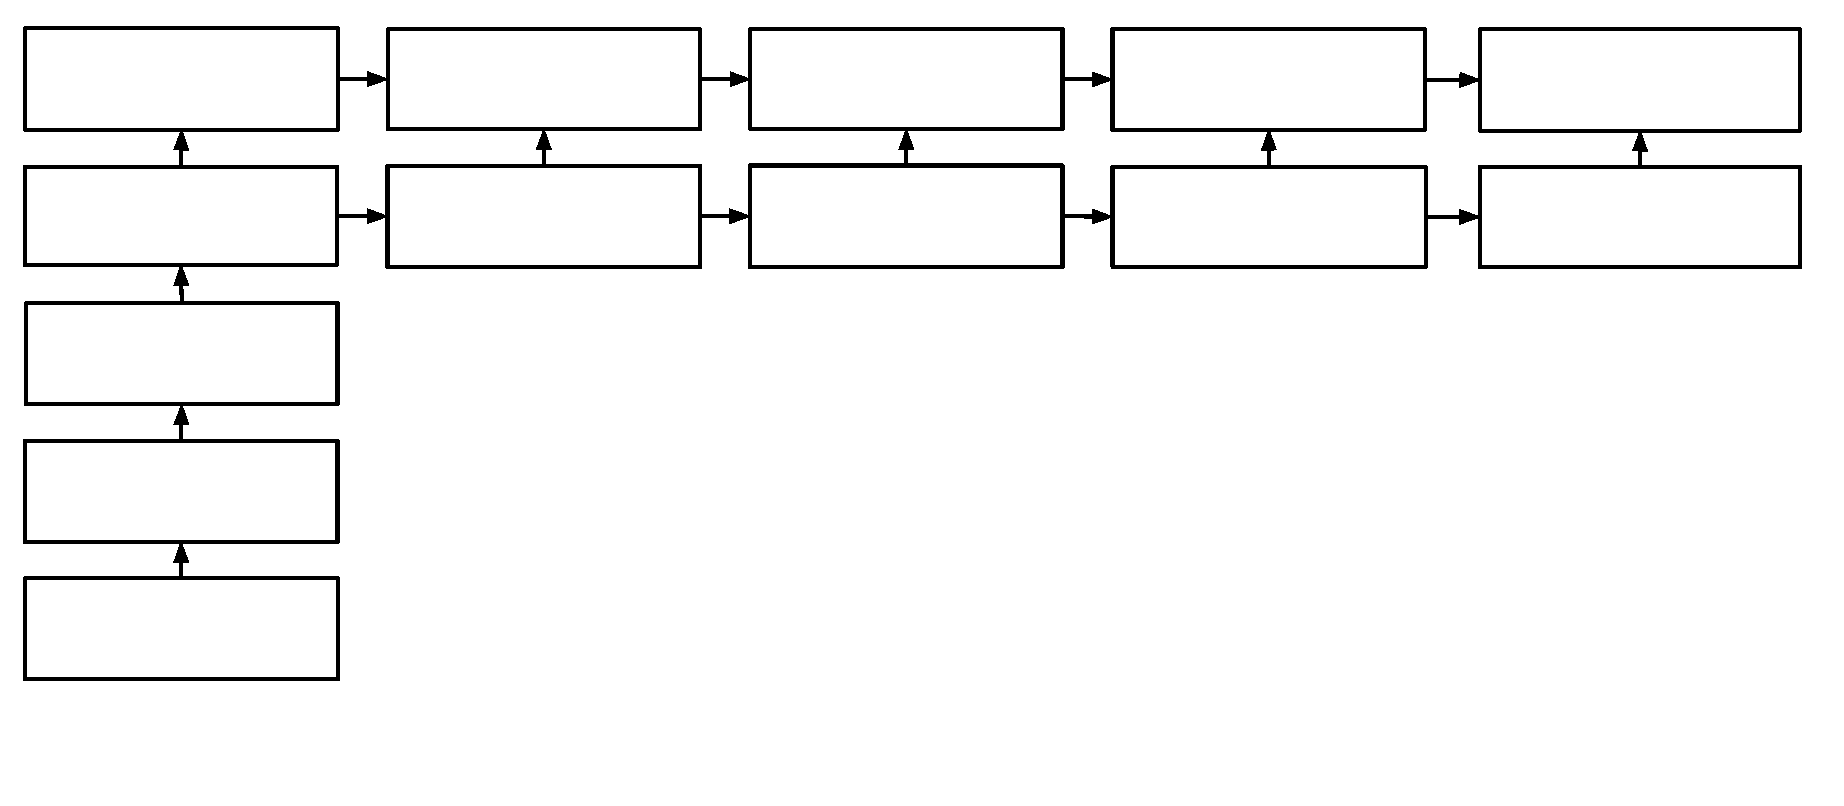
\includegraphics[width=\textwidth]{possible_pairs_of_states_of_parent_and_child_membrane}
    \caption{Possible pairs of states of parent and child membrane}
    \label{fig:possible_pairs_of_states_of_parent_and_child_membrane}
  \end{figure}

  \begin{figure}
    \def\svgwidth{\textwidth}
    \input{snapshot_of_all_membrane_states_while_simulating.pdf_tex}
    % 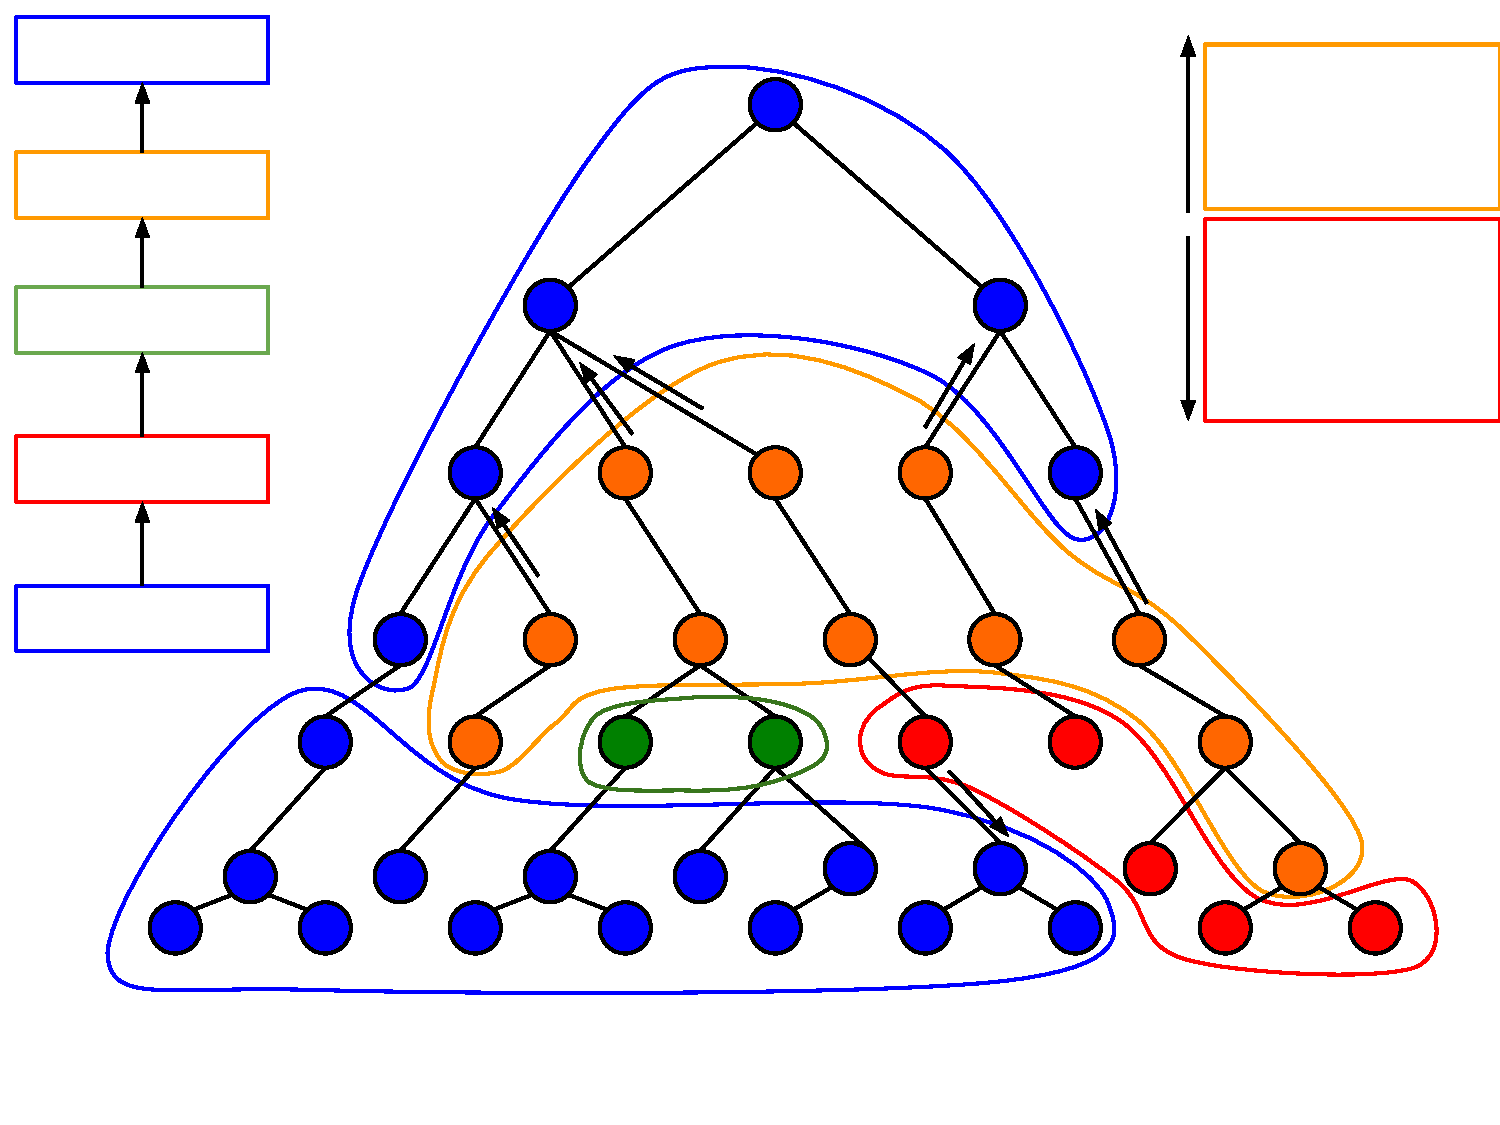
\includegraphics[width=\textwidth]{snapshot_of_all_membrane_states_while_simulating}
    \caption{Snapshot of all membrane states while simulating}
    \label{fig:snapshot_of_all_membrane_states_while_simulating}
  \end{figure}

  The pairs of possible phases of the parent and child membrane are shown in the figure \ref{fig:possible_pairs_of_states_of_parent_and_child_membrane} along with transitions between two consecutive global synchronizations - after the maximal parallel steps $i$ and $i+1$.

  In the figure \ref{fig:snapshot_of_all_membrane_states_while_simulating} the membrane structure is presented as a hierarchical structure. Every membrane is in one of four phases. It can be seen that the sending of the objects is performed in such phases that the receiving membrane is in either $RUN$ or $SYNCHRONIZE$ phase, so the received objects (marked $a^\prime$) does not interfere with rewriting.

  Another interesting idea can be seen in the figure \ref{fig:snapshot_of_all_membrane_states_while_simulating} that when a region is in the $SENDDOWN$ phase and objects are sent through the child membrane, the receiving region is in the $SYNCHRONIZE$ phase waiting for the $SYNCED$ signal, which will be sent to it when $SENDDOWN$ and $RESTORE$ phases finished.

  All membranes are nonempty during the simulation because at least the object representing the current phase is always present. By lemma~\ref{lemma:inhibitor_step} the rules with set of inhibitors can be simulated by single inhibitors.


\end{dokaz}




We have also reached this result in the accepting case by simulation of register machines.

% !TEX root = ../diz.tex
\begin{veta}
  Sequential P systems with cooperative rules and inhibitors can simulate register machines and thus equal $PsRE$.
\end{veta}


\begin{dokaz}
\label{proof:reg_by_inh}
  Suppose we have an $n$-register machine $M = (n,P,i,h)$. In our simulation we will have a membrane structure consisting of single membrane and the contents of register $j$ will be represented by the multiplicity of the object $a_j$.

  We will simulate the register machine by P system $(\Sigma, \mu, w, R)$, where:
  \begin{itemize}
    \item $\Sigma$ is an alphabet consisting of symbols that represent registers $a_1,\dots a_n$, instruction labels from the register machine $M$ and a halting symbol $\#$,
    \item $\mu$ is a membrane structure consisting of one single membrane,
    \item $w$ is initial contents of the membrane. It contains symbols for the input for the machine $a_i^{n_i}$ where $n_i$ is initial state of register with label $i$ and initial instruction label $e$.
    \item $R$ is a set of rules in the skin membrane.
  \end{itemize}
    
  For all instructions of type $(e : add(j), k, l)$ we will have rules:
  \begin{align*}
    e \rightarrow a_j|k\\
    e \rightarrow a_j|l.
  \end{align*}

  For all instructions of type $(e : sub(j), k, l)$ we will have rules:
  \begin{align*}
    e|a_j \rightarrow k\\
    e \rightarrow l|_{\neg a_j}.
  \end{align*}

  And finally halting rules:
  \begin{align*}
    h|a_j \rightarrow h|\#\text{~for all~}a\leq j\leq n,\\
    \# \rightarrow \#.
  \end{align*}

  For a configuration $(j, m_1, \dots, m_n)$ of the simulated register machine $M$ the skin membrane of the simulating P system contains a symbol $j$ and objects representing contents of registers $a_1^{m_1}, \dots, a_n^{m_n}$.

  When the halting instruction is reached, if there is an object present in the membrane, the hash symbol $\#$ is created and the rule $\# \rightarrow \#$ will be applicable forever as there is no rule to remove the symbol $\#$. If there is no object present, there is no rule to apply and computation will halt. It corresponds to the condition that all registers should be empty when halting. \qed
\end{dokaz}

\subsection{Concluding remarks} % (fold)
\label{sub:concluding_remarks_of_inhibitors}

Future plans include research other more restricted variants such as omitting cooperation in the rules or restrict the power of inhibitors.

% subsection concluding_remarks (end)

% section inhibitors (end)

\section{Active membranes} % (fold)
\label{sec:active_membranes}
In this section we study a variant of sequential systems where universality can be achieved without checking for zero by allowing membranes to be created unlimited number of times \cite{Ibarra05Active}. Such P systems are called active P systems. Contrary, if we place a limit on the number of times a membrane is created, we get a class of P systems which is only equivalent to vector addition systems, hence not universal.

In Subsection \ref{sub:active_p_systems} we will introduce membrane structure and formally define membrane configuration and active P system, because standard definitions are not convenient for our formal proofs.

The Subsection \ref{sub:termination_problems} contains two main results. The existence of an infinite computation is surprisingly\footnote{At first sight it seems to relate to the Rice's theorem, but it is not the case.} shown to be decidable.
On the other hand, the existence of a halting computation is shown to be undecidable.

\subsection{Active P systems} % (fold)
\label{sub:active_p_systems}

\begin{definition}
  \label{def:membrane_structure}
  Let $\Sigma$ be a set of objects. We denote by $\mathbb N^\Sigma$ a set of all mappings from $\Sigma$ to $\mathbb N$, so it contains all multisets of objects from $\Sigma$. A {\bf membrane configuration} is a tuple $(T, l, c)$, where:
  \begin{itemize}
    \item $T$ is a rooted tree,
    \item $l\in\mathbb N^{V(T)}$ is a mapping that assigns for each node of $T$ a number (label), where $l(r_T)=1$, so the skin membrane is always labeled with 1,
    \item $c\in(\mathbb N^\Sigma)^{V(T)}$ is a mapping that assigns for each node of $T$ a multiset of objects from $\Sigma$, so it represents the contents of the membrane.
  \end{itemize}
\end{definition}

\begin{definition}
  \label{def:active_p_system}
  An {\bf active P system} is a tuple $(\Sigma, C_0, R_1, R_2, \ldots , R_m)$, where:
  \begin{itemize}
    \item $\Sigma$ is a set of objects,
    \item $C_0$ is initial membrane configuration,
    \item $R_1,R_2,\ldots R_m$ are finite sets of rewriting rules associated with the labels $1,2,\ldots,m$ and can be of forms:
    \begin{itemize}
      \item $u\rightarrow w$, where $u\in \Sigma^+$, $w\in (\Sigma\times\{\cdot, \uparrow, \downarrow_j\})^*$ and $1\leq j\leq m$,
      \item $u\rightarrow w\delta$, where $u\in \Sigma^+$, $w\in (\Sigma\times\{\cdot, \uparrow, \downarrow_j\})^*$ and $1\leq j\leq m$,
      \item $u\rightarrow [_j v]_j$, where $u\in \Sigma^+, v\in \Sigma^*$ and $1\leq j\leq m$.
    \end{itemize}
  \end{itemize}
\end{definition}

Although rewriting rules are defined as strings, $u,v$ and $w$ represent multisets of objects from $\Sigma$. For the first two forms, each rewriting rule may specify for each object on the right side, whether it stays in the current region (we will omit the symbol $\cdot$), moves through the membrane to the parent region ($\uparrow$)
or to a specific child region ($\downarrow_j$, where $j$ is a label of a membrane). If there are more child membranes with the same label, one is chosen nondeterministically.
We denote these transfers with an arrow immediately after the symbol.
An example of such rule is the following: $abb\rightarrow ab\downarrow_2 c\uparrow c\delta$.
Symbol $\delta$ at the end of the rule means that after the application of the rule, the membrane is dissolved and its contents (objects, child membranes) are propagated to the parent membrane.
Active P systems differ from classic (passive) P systems in ability to create new membranes by rules of the third form. Such rule will create new child membrane with a given label $j$ and a given multiset of objects $v$ as its contents.

% applicable rule definition

\begin{definition}
  \label{def:applicable_rule_of_active_p_system}
  For an active P system $(\Sigma, C_0, R_1, R_2, \ldots , R_m)$, configuration $C = (T, l, c)$, membrane $d\in V(T)$ the rule $r\in R_{l(d)}$ is {\bf applicable} iff:
  \begin{itemize}
    \item $r = u\rightarrow w$ and $u\subseteq c(d)$ and for all $(a,\downarrow_k)\in w$ there exists $d_2\in V(T)$ such that $l(d_2)=k \wedge parent(d_2) = d$,
    \item $r = u\rightarrow w\delta$ and $u\subseteq c(d)$ and for all $(a,\downarrow_k)\in w$ there exists $d_2\in V(T)$ such that $l(d_2)=k \wedge parent(d_2) = d$ and $d\neq r_T$,
    \item $r = u\rightarrow [_j v]_j$ and $u\subseteq c(d)$.
  \end{itemize}
\end{definition}

In this section we assume only sequential systems, so in each step of the computation, there is one rule nondeterministically chosen among all applicable rules in all membranes to be applied as already stated in the definition \ref{def:computation_step_of_a_sequential_P_system}.

% subsection active_p_systems (end)

\subsection{Active membranes with a limit on the total number of membranes} % (fold)
\label{sub:active_membranes_with_a_limit_on_total_number_of_membranes}

For the simplicity of proofs it is convenient to introduce a variant with a global limit upon the membrane structure. We achieve this by restricting the rule application such that if the rule would result in a structure exceeding the limit, the rule will not be applicable.

\begin{definition}
  \label{def:active_p_system_with_a_limit_on_total_number_of_membranes}
  An {\bf active P system with a limit on the total number of membranes} is a tuple $\Pi = (\Sigma, L, C_0, R_1, R_2, \ldots , R_m)$, where:
  \begin{itemize}
    \item $(\Sigma, C_0, R_1, R_2, \ldots , R_m)$ is an active P system from the definition \ref{def:active_p_system},
    \item $L\in \mathbb N$ is a limit on thetotal number of membranes.
  \end{itemize}
\end{definition}
Anytime during the computation, a configuration $(T, l, c)$ is not allowed to have more than $L$ membranes, so the following invariant holds: $|V(T)|\leq L$.
This is achieved by adding a constraint for rule of the form $r = u\rightarrow [_k v]_k$, which is defined to be applicable iff $u\subseteq c(d)$ and $|V(T)|<L$. If the number of membranes is equal to $L$, there is no space for newly created membrane, so in that case such rule is not applicable.

\begin{definition}
  \label{def:applicable_rule_of_active_p_system_with_a_limit_on_total_number_of_membranes}
  For active P system with a limit on the total number of membranes $(\Sigma, L, C_0, R_1, R_2, \ldots , R_m)$, configuration $C = (T, l, c)$, membrane $d\in V(T)$ the rule $r\in R_{l(d)}$ is {\bf applicable} iff:
  \begin{itemize}
    \item $r = u\rightarrow w$ and $u\subseteq c(d)$ and $\forall (a,\downarrow_k)\in w \exists d_2\in V(T): l(d_2)=k \wedge parent(d_2) = d$,
    \item $r = u\rightarrow w\delta$ and $u\subseteq c(d)$ and $\forall (a,\downarrow_k)\in w \exists d_2\in V(T): l(d_2)=k \wedge parent(d_2) = d$ and $d\neq r_T$,
    \item $r = u\rightarrow [_j v]_j$ and $u\subseteq c(d)$ and $|V(T)|<L$.
  \end{itemize}
\end{definition}

% subsection active_membranes_with_a_limit_on_total_number_of_membranes (end)

\subsection{Termination problems} % (fold)
\label{sub:termination_problems}

In this subsection we recall the halting problem for Turing machines. The problem is to determine, given a deterministic Turing machine and an input, whether the Turing machine running on that input will halt. It is one of the first known undecidable problems. On the other hand, for non-deterministic machines, there are two possible meanings for halting. We could be interested either in:
\begin{itemize}
  \item whether there exists an infinite computation (the machine can run forever), or
  \item whether there exists a finite computation (the machine can halt).
\end{itemize}

We can ask the same questions for non-deterministic P systems.
For example we can look at the P system from the figure \ref{fig:a_single_membrane_sample_p_system}. Its computation tree (figure \ref{fig:computation_tree}) contains an infinite branch, so there exists an infinite computation with rule $r_1$ applied in each step. There is also a finite branch, so there exists a finite computation, e.g. applying rule $r_2$ results in a halting configuration.

\begin{figure}
  \centering
  \begin{minipage}{.4\textwidth}
    \begin{tikzpicture}[node distance=2mm,-triangle 45,line width=1mm]
      \tikzstyle{label of} = [above left=-5mm of #1]
      \tikzstyle{membrane} = [draw,thick,rounded corners=1cm,minimum width=2cm,minimum height=2cm,rectangle]
      \node [membrane] (m1) {
        \begin{minipage}{.8\textwidth}
          \begin{align*}
            a\\
            r_1: a\rightarrow a\\
            r_2: a\rightarrow b\\
          \end{align*}
        \end{minipage}
      };
    \end{tikzpicture}
    \captionof{figure}{A single-membrane sample P system}
    \label{fig:a_single_membrane_sample_p_system}
  \end{minipage}
  \hspace{.08\textwidth}
  \begin{minipage}{.5\textwidth}
    \centering
    \begin{tikzpicture}[level distance=2cm,sibling distance=4cm,-triangle 45]
      \tikzstyle{every node} = [circle,draw]
      \node (Root) {a}
        child {
          node {a}
          child {
            node [draw=none] {$\ldots$}
            edge from parent node [above left,draw=none] {$r_1$}
          }
          child { node {b} edge from parent node [above right,draw=none] {$r_2$} }
          edge from parent node [above left,draw=none] {$r_1$}
        }
        child { node {b} edge from parent node [above right,draw=none] {$r_2$} };
    \end{tikzpicture}  
    \captionof{figure}{The computation tree of the P system from the figure \ref{fig:a_single_membrane_sample_p_system}}
    \label{fig:computation_tree}
  \end{minipage}
\end{figure}

We will prove the (un)decidability of these problems on active P systems with limit on the total number of membranes. The results are quite interesting, because:

\begin{veta}
  Sequential active P systems with limit on the total number of membranes are universal.
\end{veta}

\begin{dokaz}
  The proof of this theorem for sequential active P systems in \cite{Ibarra05Active} uses simulation of register machines and during the simulation, every configuration has at most three membranes. Hence the active P system with limit on the total number of membranes exists (e.g. with $L=3$), so the universality holds.
  \qed
\end{dokaz}

\subsubsection{Existence of infinite computation} % (fold)
\label{ssub:existence_of_infinite_computation}

We will propose an algorithm for deciding existence of infinite computation. Basic idea is to consider the minimal coverability graph (\cite{Rozenberg93MinimalCoverabilityGraph}), where nodes are configurations and an edge leads from the configuration $C_1$ to the configuration $C_2$, whenever there is a rule applicable in $C_1$, which results in $C_2$. The construction in \cite{Rozenberg93MinimalCoverabilityGraph} is performed on Petri nets, where the configuration consists just of a vector of natural numbers. The situation is the same for single-membrane sequential P systems. We need to modify the construction for active P systems.

\begin{definition}
  A configuration $C_2 = (T_2, l_2, c_2)$ {\bf covers} configuration $C_1 = (T_1, l_1, c_1)$ iff $\exists$ isomorphism $f: T_1\rightarrow T_2$ preserving membrane labels and contents: $\forall d\in T_1$ the following properties hold: $l_1(d)=l_2(f(d))\wedge c_1(d)\subseteq c_2(f(d))$. We will denote this with $C_1\leq C_2$.
\end{definition}

\begin{figure}
  \begin{tikzpicture}[node distance=2mm,line width=1mm]
    \tikzstyle{label of} = [above left=-5mm of #1]
    \tikzstyle{membrane} = [draw,thick,rounded corners=1cm,minimum width=2cm,minimum height=2cm,rectangle]
    \node [membrane] (m1) {
      \begin{minipage}{.42\textwidth}
        \begin{align*}
          a\\
        \end{align*}
      \end{minipage}
    };
    \node [label of=m1] (l1) {1};
    \node [below=1mm of m1] (c1) {$C_1$};
    \node [membrane,right=.08\textwidth of m1] (m2) {
      \begin{minipage}{.42\textwidth}
        \begin{align*}
          a,b\\
        \end{align*}
      \end{minipage}
    };
    \node [label of=m2] (l2) {1};
    \node [below=1mm of m2] (c2) {$C_2$};
    \node [membrane,below=.08\textwidth of c1] (m3) {
      \begin{minipage}{.42\textwidth}
        \begin{align*}
          a\\
        \end{align*}
      \end{minipage}
    };
    \node [label of=m3] (l3) {2};
    \node [below=1mm of m3] (c3) {$C_3$};
    \node [membrane,below=.08\textwidth of c2] (m4) {
      \begin{tikzpicture}
        \node (m4a) {$a$};
        \tikzstyle{label of} = [above left=-15mm of #1]
        \node [membrane,minimum width=3cm,right=1mm of m4a] (m5) {a};
        \node [label of=m5] (l5) {1};
      \end{tikzpicture}      
    };
    \node [label of=m4] (l4) {1};
    \node [below=1mm of m4] (c4) {$C_4$};
  \end{tikzpicture}
  \caption{Sample membrane configurations}
  \label{fig:sample_membrane_configurations}
\end{figure}

\begin{example}
  In the figure \ref{fig:sample_membrane_configurations} there are four membrane configuration. $C_1\leq C_2$, because the membrane structures consists of one membrane, so the corresponding trees are isomorphic. The label is the same and the contents of the membrane in $C_1$ is a subset of the contents of the membrane in $C_2$. It does not have to be a proper subset, i.e. $C_1\leq C_1$.$C_1$ and $C_3$ are incomparable, because the label is different, so neither $C_1\leq C_3$ nor $C_3\leq C_1$ holds. $C_1$ and $C_4$ are also incomparable, because the trees of their membrane structure are not isomorphic.
\end{example}

We will now follow with a proof of an important property of the covering relation - that it maintains rule applicability.

\begin{lemma}
\label{rule_applicability_lemma}
  For sequential active P system with limit on the total number of membranes, if $C_2 = (T_2, l_2, c_2)$ {\bf covers} configuration $C_1 = (T_1, l_1, c_1)$, then there is an isomorphism $f: T_1\rightarrow T_2$ such that if a rule $r$ is applicable in membrane $d\in T_1$, then $r$ is applicable in $f(d)$.
\end{lemma}

\begin{dokaz}
  Suppose $r$ is applicable in $d$. Then the left side $u$ of the rule $r$ is contained within the contents of the membrane $u\subseteq c_1(d)$. Because $C_1\leq C_2$, then there is an isomorphism $f:T_1\rightarrow T_2$ such that $c_1(d)\subseteq c_2(f(d))$ and then $u\subseteq c_2(f(d))$.

  There are three possible forms of the rule $r$.
  \begin{itemize}
    \item If $r = u\rightarrow w$, then, because $r$ is applicable in $d$, $\forall (a,\downarrow_k)\in w \exists d_2\in V(T_1): l_1(d_2)=k \wedge parent_{T_1}(d_2) = d$. Because $C_1\leq C_2$, then for $f(d_2)\in V(T_2)$ the following holds: $l_2(f(d_2)) = l_1(d_2) = k$ and $parent_{T_2}(f(d_2) = f(d)$. Hence $r$ is applicable in $f(d)$.
    \item If $r = u\rightarrow w\delta$, then $d\neq r_{T_1}$. Since $f$ is an isomorphism, then also $f(d)\neq r_{T_2}$. Other properties follows from the previous case.
    \item If $r = u\rightarrow [_k v]_k$, then $|V(T_1)|<L$. Isomorphism preserves number of nodes, hence $|V(T_2)| = |V(T_1)| < L$ and $r$ is applicable in $f(d)$. \qed
  \end{itemize}
\end{dokaz}

Now, we will define the encoding of a configuration $C = (T, l, c)$ into a tuple of integers.

A membrane $d\in T$ will be encoded as $(n+m)$-tuple $enc(d)\in\mathbb N^{(n+m)}$, where first $n$ numbers will be actual counts of objects and next $m$ numbers will encode the membrane label:
\[
  enc(d)_{i} =
  \begin{cases}
    c(d)(a_i) & \text{if}\ i\leq n\\
    0 & \text{if}\ n<i\leq m\wedge i-n\neq l(d)\\
    1 & \text{if}\ n<i\leq m\wedge i-n=l(d)
  \end{cases}
\].

The entire tree will be encoded into concatenated sequences of encoded nodes in the preorder traversal order. This sequence is then padded with zeroes to have length $(n+m)L$ as that is the maximal length of encoded tree.

Since there are only finitely many non-isomorphic trees with at most $L$ nodes (\cite{Cayley1881RootedTrees}), there is a constant $z$ such that we can uniquely assign the tree an order number $o(T) \leq z$.

The entire configuration will be encoded in tuple which consists of $z$ parts. All but the part with index $o(T)$ will contain just zeros. The part with index $o(T)$ will contain the encoding of the tree.

\begin{example}
  Consider $L=2$. There are just two rooted trees with at most 2 nodes. We can define $o(T)=1$ for the single-node tree and $o(T)=2$ for the tree with a root and one child. So the encodings of configurations from figure \ref{fig:sample_membrane_configurations} contain two parts. Configurations $C_1, C_2$, and $C_3$ consists of one membrane, so their $o(T)=1$ and the second part is filled with zeroes. Configuration $C_4$ contains two membranes, so its $o(T)=2$ and the first part of its encoding will be filled with zeroes. 
  \begin{itemize}
    \item $enc(C_1)=\overbrace{\underbrace{1}_{c(a)}\underbrace{0}_{c(b)}\underbrace{1}_{l=1?}\underbrace{0}_{l=2?}}^{\mathclap{\text{skin membrane encoded}}}\underbrace{0000}_\text{padding to fit $(n+m)L$}\overbrace{00000000}^{\mathclap{\text{second part filled with zeroes}}}$,
    \item $end(C_2)=1110000000000000$,
    \item $enc(C_3)=1001000000000000$,
    \item $enc(C_4)=00000000\overbrace{1010}^{\mathclap{\text{skin membrane encoded}}}\underbrace{1010}_{\mathclap{\text{child membrane encoded}}}$
  \end{itemize}
\end{example} 

We will now show that comparing two encodings corresponds to covering of two configurations. Recall that configurations are encoded into tuples of integers, so the comparison is performed position by position.

\begin{lemma}
\label{encoding_lemma}
  For configurations $C_1 = (T_1, l_1, c_1)$ and $C_2 = (T_2, l_2, c_2)$, $enc(C_1) \leq enc(C_2)\Rightarrow C_1\leq C_2$.
\end{lemma}

\begin{dokaz}
  Both $enc(C_1)$ and $enc(C_2)$ contain $z$ parts and exactly one part which contains non-zero values. The non-zero part of $enc(C_1)$ must be non-zero also in $enc(C_2)$, because $enc(C_1)\leq enc(C_2)$. Then $o(T_1)=o(T_2)$, so the trees are isomorphic. Suppose there is an isomorphism $f:T_1\rightarrow T_2$. For every membrane $d\in T_1$, $l_1(d)=l_2(f(d))$ and $c_1(d)\subseteq c_2(f(d))$. Hence, $C_1\leq C_2$.
  \qed
\end{dokaz}

\begin{lemma}
\label{infinite_sequence_of_configurations_lemma}
  For sequential active P system with limit on the total number of membranes $L$ for every infinite sequence of configurations $\{C_i\}_{i=0}^\infty\exists i<j: C_i\leq C_j$.
\end{lemma}

\begin{dokaz}
  Suppose an infinite sequence $\{enc(C_i)\}_{i=0}^\infty$. We use a variation of Dickson's lemma (\cite{Figueira11Dickson}): Every infinite sequence of tuples from $\mathbb N^k$ contains an increasing pair. Applied to our sequence, there are two positions $i<j: enc(C_i)\leq enc(C_j)$. From lemma \ref{encoding_lemma}, $C_i\leq C_j$.
  \qed
\end{dokaz}

\begin{veta}
  Existence of infinite computation for active P systems with limit on the total number of membranes is decidable.
\end{veta}

\begin{dokaz}
  The algorithm for deciding the problem will traverse the reachability graph. When it encounters a configuration that covers another configuration, from lemma \ref{rule_applicability_lemma} follows that the same rules can be applied repeatedly, so the algorithm will halt with the answer YES.
  Otherwise, the algorithm will answer NO.
  Algorithm will always halt, because if there was an infinite computation, from lemma \ref{infinite_sequence_of_configurations_lemma} there would be two increasing configurations which is already covered in the YES case.
  \qed
\end{dokaz}

% subsubsection existence_of_infinite_computation (end)

\subsubsection{Existence of halting computation} % (fold)
\label{ssub:existence_of_halting_computation}

In this subsection we will focus on the opposite problem: whether there is a computation that is halting. Recall that halting computation has no applicable rule in the last configuration.
First, we will reduce this problem to the reachability problem. It is a problem of determining, for a given configuration $C$, whether there exists a computation from $C_0$ to $C$. The reachability of active P systems can be then reduced to the reachabililty of register machines, which is undecidable.

For a given P system $\Pi$ and a target configuration $C$ we will construct a P system $\Pi^\prime$ such that there is a halting computation of $\Pi^\prime\Leftrightarrow\linebreak C$ is reachable for $\Pi$. Suppose $\Pi = (\Sigma, C_0, R_1, \ldots R_m)$ and $C = (T, l, c)$. Then we will construct $\Pi^\prime = (\Sigma^\prime, C_0^\prime, R_1^\prime, \ldots R_m^\prime)$, where:

\begin{itemize}
  \item $\Sigma^\prime = \Sigma\cup\{\xi_d|d\in V(T)\}$,
  \item $C_0^\prime = (T, l, c^\prime)$, where $\forall d\in V(T)\setminus r_T: c^\prime(d) = c(d)$ and $c^\prime(r_T) = c(r_T)\cup\{\xi_{r_T}\}$,
  \item $\forall i\in\{1\ldots m\}: R_i^\prime = R_i\cup\{\xi_d c(d)\rightarrow\xi_{d^\prime}\downarrow_{l(d^\prime)}|d,d^\prime\in V(T),l(d)=i,parent(d^\prime)=d\}$.
\end{itemize}

The $\xi_d$ objects are called verifiers, they are intended to verify if the contents of the membrane corresponds to the contents in the target configuration $C$. After this verification it descends down into child membranes for the verification of other parts of the membrane structure.
Initially, there is an object $\xi_{r_T}$ in the skin membrane. Verification is performed in the rule $\xi_d c(d)\rightarrow\xi_{d^\prime}\downarrow_{l(d^\prime)}$, where on the right side there is $\xi_{d^\prime}$ object for every child membrane $d^\prime$ in the target configuration $C$.

The construction is not complete. The system should not be able to halt unless the verification takes place. That is why we introduce a new object $\omega$ to each membrane with a rule $\omega\rightarrow\omega$ and the verifier will erase them with rule $\xi_d\omega c(d)\rightarrow\xi_{d^\prime}\downarrow_{l(d^\prime)}$. One application of this rule will erase the $\omega$ object and propagate proper $\xi$ object to every child membrane. We also need to ensure that newly created membranes contain the $\omega$ object, so we replace every rule for membrane creation $u\rightarrow [_k v]_k$ with $u\rightarrow [_k v\omega]_k$.

\begin{figure}
  \begin{tikzpicture}[node distance=2mm,line width=1mm]
    \tikzstyle{label of} = [above left=-5mm of #1]
    \tikzstyle{membrane} = [draw,thick,rounded corners=1cm,minimum width=2cm,minimum height=2cm,rectangle]
    \node [membrane] (m1) {
      \begin{minipage}{.2\textwidth}
        \begin{align*}
          a\\
          a\rightarrow [a]_2\\
        \end{align*}
      \end{minipage}
    };
    \node [label of=m1] (l1) {1};
    \node [below=1mm of m1] (pi1) {$\Pi_1$};
    \node [membrane,right=.04\textwidth of m1] (m2) {$a$};
    \node [label of=m2] (l2) {1};
    \node [below=1mm of m2] (c0) {$C_0$};
    \node [membrane,right=.04\textwidth of m2] (m3) {
      \begin{tikzpicture}
        \tikzstyle{label of} = [above left=-15mm of #1]
        \node [membrane] (m4) {a};
        \node [label of=m4] (l4) {2};
      \end{tikzpicture}      
    };
    \node [label of=m3] (l3) {1};
    \node [below=1mm of m3] (c) {$C_1$};
    \node [membrane,right=.04\textwidth of m3] (m5) {
      \begin{tikzpicture}
        \tikzstyle{label of} = [above left=-15mm of #1]
        \node [membrane] (m6) {};
        \node [label of=m6] (l6) {2};
      \end{tikzpicture}      
    };
    \node [label of=m5] (l5) {1};
    \node [below=1mm of m5] (c) {$C_2$};
  \end{tikzpicture}
  \caption{Example P system $\Pi_1$}
  \label{fig:example_p_system_pi_1}
\end{figure}

\begin{figure}
  \begin{tikzpicture}[node distance=2mm,line width=1mm]
    \tikzstyle{label of} = [above left=-5mm of #1]
    \tikzstyle{membrane} = [draw,thick,rounded corners=1cm,minimum width=2cm,minimum height=2cm,rectangle]
    \node [membrane] (m1) {
      \begin{minipage}{.24\textwidth}
        \begin{align*}
          a\\
        \end{align*}
      \end{minipage}
    };
    \node [label of=m1] (l1) {1};
    \node [below=1mm of m1] (c0) {$C_0$};
    \node [membrane,right=.3\textwidth of m1] (m2) {
      \begin{tikzpicture}
        \tikzstyle{label of} = [above left=-15mm of #1]
        \node [membrane] (m3) {a};
        \node [label of=m3] (l3) {2};
      \end{tikzpicture}      
    };
    \node [label of=m2] (l2) {1};
    \draw (m1) edge [-triangle 45,thin,shorten >=3mm,shorten <=3mm] node [above] {$a\rightarrow [a]_2$} (m2);
  \end{tikzpicture}
  \caption{Computation of $\Pi_1$}
  \label{fig:computation_of_pi_1}
\end{figure}

\begin{figure}
  \begin{tikzpicture}[node distance=2mm,line width=1mm]
    \tikzstyle{label of} = [above left=-5mm of #1]
    \tikzstyle{membrane} = [draw,thick,rounded corners=1cm,minimum width=2cm,minimum height=2cm,rectangle]
    \node [membrane] (m1) {$a\xi_{d_1}\omega$};
    \node [label of=m1] (l1) {1};
    \node [below=1mm of m1] (c0) {$C^\prime_0$};
    \node [membrane,right=.3\textwidth of m1] (m2) {
      \begin{tikzpicture}
        \node (m4a) {$\xi_{d_1} \omega$};
        \tikzstyle{label of} = [above left=-15mm of #1]
        \node [membrane,minimum width=3cm,right=1mm of m4a] (m3) {$a\omega$};
        \node [label of=m3] (l3) {2};
      \end{tikzpicture}      
    };
    \node [label of=m2] (l2) {1};
    \node [membrane,below=.2\textwidth of m1] (m4) {
      \begin{tikzpicture}
        \tikzstyle{label of} = [above left=-15mm of #1]
        \node [membrane,minimum width=3cm] (m5) {$a\xi_{d_2}\omega$};
        \node [label of=m5] (l5) {2};
      \end{tikzpicture}      
    };
    \node [label of=m4] (l4) {1};
    \node [membrane,right=.2\textwidth of m4] (m6) {
      \begin{tikzpicture}
        \tikzstyle{label of} = [above left=-15mm of #1]
        \node [membrane,minimum width=3cm] (m7) {};
        \node [label of=m7] (l7) {2};
      \end{tikzpicture}      
    };
    \node [label of=m6] (l6) {1};
    \draw (m1) edge [-triangle 45,thin,shorten >=3mm,shorten <=3mm] node [above] {$a\rightarrow [a\omega]_2$} (m2);
    \draw (m2) edge [-triangle 45,thin,shorten >=3mm,shorten <=3mm] node [sloped,above] {$\xi_{d_1}\omega\rightarrow\xi_{d_2}\downarrow_2$} (m4);
    \draw (m4) edge [-triangle 45,thin,shorten >=3mm,shorten <=3mm] node [above] {$\xi_{d_2}a\omega\rightarrow \eps$} (m6);
  \end{tikzpicture}
  \caption{Computation of $\Pi^\prime_1$}
  \label{fig:computation_of_pi_prime_1}
\end{figure}

\begin{figure}
  \begin{tikzpicture}[node distance=2mm,line width=1mm]
    \tikzstyle{label of} = [above left=-5mm of #1]
    \tikzstyle{membrane} = [draw,thick,rounded corners=1cm,minimum width=2cm,minimum height=2cm,rectangle]
    \node [membrane] (m1) {$a\xi_{d_1}\omega$};
    \node [label of=m1] (l1) {1};
    \node [below=1mm of m1] (c0) {$C^\prime_0$};
    \node [membrane,right=.3\textwidth of m1] (m2) {
      \begin{tikzpicture}
        \node (m4a) {$\xi_{d_1} \omega$};
        \tikzstyle{label of} = [above left=-15mm of #1]
        \node [membrane,minimum width=3cm,right=1mm of m4a] (m3) {$a\omega$};
        \node [label of=m3] (l3) {2};
      \end{tikzpicture}      
    };
    \node [label of=m2] (l2) {1};
    \node [membrane,below=.2\textwidth of m1] (m4) {
      \begin{tikzpicture}
        \tikzstyle{label of} = [above left=-15mm of #1]
        \node [membrane,minimum width=3cm] (m5) {$a\xi_{d_2}\omega$};
        \node [label of=m5] (l5) {2};
      \end{tikzpicture}      
    };
    \node [label of=m4] (l4) {1};
    \node [membrane,right=.2\textwidth of m4] (m6) {
      \begin{tikzpicture}
        \tikzstyle{label of} = [above left=-15mm of #1]
        \node [membrane,minimum width=3cm] (m7) {$a$};
        \node [label of=m7] (l7) {2};
      \end{tikzpicture}      
    };
    \node [label of=m6] (l6) {1};
    \draw (m1) edge [-triangle 45,thin,shorten >=3mm,shorten <=3mm] node [above] {$a\rightarrow [a\omega]_2$} (m2);
    \draw (m2) edge [-triangle 45,thin,shorten >=3mm,shorten <=3mm] node [sloped,above] {$\xi_{d_1}\omega\rightarrow\xi_{d_2}\downarrow_2$} (m4);
    \draw (m4) edge [-triangle 45,thin,shorten >=3mm,shorten <=3mm] node [above] {$\xi_{d_2}\omega\rightarrow \eps$} (m6);
  \end{tikzpicture}
  \caption{Computation of $\Pi^\prime_2$}
  \label{fig:computation_of_pi_prime_2}
\end{figure}

\begin{example}
  An example P system $\Pi_1 = (\{a,b\}, C_0, \{a\rightarrow [a]_2\}, \{\})$ is depicted in the Figure \ref{fig:example_p_system_pi_1}. The target configuration $C_1$ with the membrane structure consisting of the root membrane $d_1$ with label $1$ and its child membrane $d_2$ with label $2$ can be easily reached by applying the rule $a\rightarrow [a]_2$ in the skin membrane. This computation is shown in the Figure \ref{fig:computation_of_pi_1}.

  We will construct a corresponding P system $\Pi^\prime_1=(\{a,b,\xi_{d_1},\xi_{d_2},\omega\}, C^\prime_0, \linebreak\{a\rightarrow [a]_2,\xi_{d_1}\omega\rightarrow\xi_{d_2},\omega\rightarrow\omega\}, \{\xi_{d_2}a\omega\rightarrow\eps,\omega\rightarrow\omega\})$. The initial configuration $C^\prime_0$ is shown in the Figure \ref{fig:computation_of_pi_prime_1}. There is also a halting computation which corresponds to the computation of $\Pi_1$ that reaches the target configuration $C_1$.
\end{example}

\begin{example}
There is still a problem. We actually check, whether a target configuration is contained within the current configuration. If our target configuration is $C_2$ from the Figure \ref{fig:example_p_system_pi_1}, the resulting P system $\Pi^\prime_2=(\{a,b,\xi_{d_1},\xi_{d_2},\omega\}, C^\prime_0, \{a\rightarrow [a]_2,\xi_{d_1}\omega\rightarrow\xi_{d_2},\omega\rightarrow\omega\}, \{\xi_{d_2}\omega\rightarrow\eps,\omega\rightarrow\omega\})$ will have the same halting computation shown in the Figure \ref{fig:computation_of_pi_prime_2} although the configuration $C_2$ cannot be reached.  
\end{example}

If there are additional objects which cannot be erased, so the target configuration cannot be reached, we need to ensure $\Pi^\prime$ will not halt. We will add a rule $a\rightarrow a$ to each membrane for each object $a\in\Sigma$, so $\Pi^\prime$ can halt only if all objects are erased. This modification renders the computation in the Figure \ref{fig:computation_of_pi_prime_2} as not halting.

The last issue to solve is the dissolution. It is still possible that in the middle of the verifying, some of already verified membranes got dissolved and all yet unverified membranes will be successfully verified causing $\Pi^\prime$ to halt, although without that dissolution it would be unable to reach $C$.

\begin{figure}
  \begin{tikzpicture}[node distance=2mm,line width=1mm]
    \tikzstyle{label of} = [above left=-5mm of #1]
    \tikzstyle{membrane} = [draw,thick,rounded corners=1cm,minimum width=2cm,minimum height=2cm,rectangle]
    \node [membrane] (m1) {
      \begin{tikzpicture}
        \tikzstyle{label of} = [above left=-15mm of #1]
        \node [membrane] (m2) {
          \begin{minipage}{.2\textwidth}
            \begin{align*}
              a\\
              a\rightarrow \delta\\
            \end{align*}
          \end{minipage}
        };
        \node [label of=m2] (l2) {2};
      \end{tikzpicture}

    };
    \node [label of=m1] (l1) {1};
    \node [below=1mm of m1] (pi1) {$\Pi_3$};
    \node [membrane,right=.08\textwidth of m1] (m3) {$a$};
    \node [label of=m3] (l3) {1};
    \node [below=1mm of m3] (c0) {$C_0$};
    \node [membrane,right=.08\textwidth of m3] (m4) {
      \begin{tikzpicture}
        \tikzstyle{label of} = [above left=-15mm of #1]
        \node [membrane] (m5) {};
        \node [label of=m5] (l5) {2};
      \end{tikzpicture}      
    };
    \node [label of=m4] (l4) {1};
    \node [below=1mm of m4] (c) {$C_3$};
  \end{tikzpicture}
  \caption{Example P system $\Pi_3$}
  \label{fig:example_p_system_pi_3}
\end{figure}

\begin{figure}
  \begin{tikzpicture}[node distance=2mm,line width=1mm]
    \tikzstyle{label of} = [above left=-5mm of #1]
    \tikzstyle{membrane} = [draw,thick,rounded corners=1cm,minimum width=2cm,minimum height=2cm,rectangle]
    \node [membrane] (m1) {
      \begin{tikzpicture}
        \tikzstyle{label of} = [above left=-15mm of #1]
        \node [membrane] (m2) {a};
        \node [label of=m2] (l2) {2};
      \end{tikzpicture} 
    };
    \node [label of=m1] (l1) {1};
    \node [below=1mm of m1] (c0) {$C_0$};
    \node [membrane,right=.3\textwidth of m1] (m3) {};
    \node [label of=m3] (l3) {1};
    \draw (m1) edge [-triangle 45,thin,shorten >=3mm,shorten <=3mm] node [above] {$a\rightarrow \delta$} (m3);
  \end{tikzpicture}
  \caption{Computation of $\Pi_3$}
  \label{fig:computation_of_pi_3}
\end{figure}

\begin{figure}
  \begin{tikzpicture}[node distance=2mm,line width=1mm]
    \tikzstyle{label of} = [above left=-5mm of #1]
    \tikzstyle{membrane} = [draw,thick,rounded corners=1cm,minimum width=2cm,minimum height=2cm,rectangle]
    \node [membrane] (m1) {
      \begin{tikzpicture}
        \node (m1a) {$\xi_{d_1} \omega$};
        \tikzstyle{label of} = [above left=-15mm of #1]
        \node [membrane,minimum width=3cm,right=1mm of m1a] (m2) {$a\omega$};
        \node [label of=m2] (l2) {1};
      \end{tikzpicture}
    };
    \node [label of=m1] (l1) {1};
    \node [below=1mm of m1] (c0) {$C^\prime_0$};
    \node [membrane,right=.25\textwidth of m1] (m3) {
      \begin{tikzpicture}
        \tikzstyle{label of} = [above left=-15mm of #1]
        \node [membrane,minimum width=3cm] (m4) {$a\xi_{d_2}\omega$};
        \node [label of=m4] (l4) {1};
      \end{tikzpicture}      
    };
    \node [label of=m3] (l3) {1};
    \node [membrane,below=.2\textwidth of m1] (m5) {$\xi_{d_2}\omega$};
    \node [label of=m5] (l5) {1};
    \node [membrane,right=.35\textwidth of m5] (m6) {};
    \node [label of=m6] (l6) {1};
    \draw (m1) edge [-triangle 45,thin,shorten >=3mm,shorten <=3mm] node [above] {$\xi_{d_1}\omega\rightarrow\xi_{d_2}\downarrow_1$} (m3);
    \draw (m3) edge [-triangle 45,thin,shorten >=3mm,shorten <=3mm] node [sloped,above] {$a\rightarrow \delta$} (m5);
    \draw (m5) edge [-triangle 45,thin,shorten >=3mm,shorten <=3mm] node [above] {$\xi_{d_2}\omega\rightarrow \eps$} (m6);
  \end{tikzpicture}
  \caption{Computation of $\Pi^\prime_3$}
  \label{fig:computation_of_pi_prime_3}
\end{figure}

\begin{example}
  In the figure \ref{fig:example_p_system_pi_3} there is a P system $\Pi_3 = (\{a\}, C_0, \{a\rightarrow \delta\})$. The target configuration $C_3$ cannot be reached, because erasing $a$ will also dissolve the child membrane. We cannot keep the membrane while getting rid of $a$. The only possible computation is depicted in the Figure \ref{fig:computation_of_pi_3}.

  The resulting P system will be $\Pi^\prime_3 = (\{a,\xi_{d_1},\xi_{d_2},\omega\}, C^\prime_0, \{a\rightarrow \delta, a\rightarrow a, \linebreak\xi_{d_1}\omega\rightarrow\xi_{d_2}, \xi_{d_2}\omega\rightarrow\eps, \omega\rightarrow\omega\})$. Its initial configuration $C^\prime_0$ and the halting computation are shown in the Figure \ref{fig:computation_of_pi_prime_3}.
\end{example}

We need to ensure all dissolution happen before the verification takes place.
We will add a new object $\sigma$, which stands as a footprint object. It will be created as a result of the verification rule $\xi_d\omega c(d)\rightarrow\sigma\xi_{d^\prime}\downarrow_{l(d^\prime)}$. If a membrane is dissolved after it was verified, then two $\sigma$s will meet in the same membrane, because the parent membrane also contains $\sigma$ as it had been verified before. We will add a rule $\sigma\sigma\rightarrow\sigma\sigma$ to prevent $\Pi^\prime$ from halting.

The final construct is:

\begin{itemize}
  \item $\Sigma^\prime = \Sigma\cup\{\omega, \sigma\}\cup\{\xi_d|d\in V(T)\}$,
  \item $C_0^\prime = (T, l, c^\prime)$, where $\forall d\in V(T)\setminus r_T: c^\prime(d) = c(d)\cup\{\omega\}$ and $c^\prime(r_T) = c(r_T)\cup\{\omega,\xi_{r_T}\}$,
  \item $\forall i\in\{1\ldots m\}: R_i^\prime = \{r|r\in R_i,r = u\rightarrow w\vee r = u\rightarrow w\delta\}\cup\linebreak\{u\rightarrow [_k v\omega]_k|u\rightarrow [_k v]_k\in R_i\}\cup\{a\rightarrow a|a\in\Sigma\}\cup\{\sigma\sigma\rightarrow\sigma\sigma,\omega\rightarrow\omega\}\cup\linebreak\{\xi_d\omega c(d)\rightarrow\sigma\xi_{d^\prime}\downarrow_{l(d^\prime)}|d,d^\prime\in V(T),l(d)=i,parent(d^\prime)=d\}$.
\end{itemize}

We need to prove two implications in order to formally prove correctness of this construction.

\begin{lemma}
\label{if_reachable_then_halting_lemma}
  If $C$ is reachable for $\Pi$ then there is a halting computation of $\Pi^\prime$.
\end{lemma}

\begin{dokaz}
  Consider a computation $\Pi$ with $C$ as the last configuration. For $\Pi^\prime$ there is a corresponding computation as the rules of $\Pi$ are included in $\Pi^\prime$ with an exception of the rule $u\rightarrow [_k v]_k$, which has a corresponding rule with the same left side: $u\rightarrow [_k v\omega]_k$. The corresponding computation of $\Pi^\prime$ will result in a configuration, where in every membrane $d$, the contents will be $\omega c(d)$, and the skin membrane will contain an additional $\xi_{r_T}$. Then the cascade of applications of the rule $\xi_d\omega c(d)\rightarrow\sigma\xi_{d^\prime}\downarrow_{l(d^\prime)}$ can start in the skin membrane, cascading down from parents to children until all the membranes applied that rule. The objects $\omega c(d)$ will be replaced by $\sigma$ and the computation will halt. \qed
\end{dokaz}

The other direction of the implication is more complicated, so the following lemmas will state some properties about computations of $\Pi$ and $\Pi^\prime$.

\begin{lemma}
\label{no_dissolving_after_check_lemma}
  For all halting computations of $\Pi^\prime$ there is no rule of form $u\rightarrow w\delta$ applied in the membrane $d^\prime$ after the application of rule $\xi_d\omega c(d)\rightarrow\sigma\xi_{d^\prime}\downarrow_{l(d^\prime)}$ in membrane $d=parent(d^\prime)$.
\end{lemma}

\begin{dokaz}
  After the application of the rule $\xi_d\omega c(d)\rightarrow\sigma\xi_{d^\prime}\downarrow_{l(d^\prime)}$, the object $\sigma$ remains in the membrane. There is no possible interaction of $\sigma$ with other objects, only with another $\sigma$. If a child membrane $d^\prime$ is dissolved with a rule $u\rightarrow w\delta$, then two objects $\sigma$ will meet in the membrane $d$ and the computation will not halt, which contradicts the fact that the computation is halting. \qed
\end{dokaz}

\begin{lemma}
\label{no_creating_new_membrane_after_check_lemma}
  For all halting computations of $\Pi^\prime$ there is no rule of form $u\rightarrow [_k v\omega]_k$ applied in the membrane $d^\prime$ after the application of rule $\xi_d\omega c(d)\rightarrow\sigma\xi_{d^\prime}\downarrow_{l(d^\prime)}$.
\end{lemma}

\begin{dokaz}
  After the application of the rule $r = \xi_d\omega c(d)\rightarrow\sigma\xi_{d^\prime}\downarrow_{l(d^\prime)}$ in membrane $d$, there will not be any of $\xi$ objects present in the membrane, because they are only sent into child membranes, which cannot be dissolved, because of Lemma \ref{no_dissolving_after_check_lemma}. So there will be no more of rule $r$ applied in membrane $d$. The newly created membrane will never receive any of $\xi$ objects, so the object $\omega$ will never be erased and the computation will not halt, which contradicts the fact that the computation is halting. \qed
\end{dokaz}

\begin{lemma}
\label{check_at_last_lemma}
  If a halting computation of $\Pi^\prime$ exists then there is a halting computation, where for every membrane $d\in V(T)$ in the target configuration $C=(T,l,c)$ the last rule used is $r = \xi_d\omega c(d)\rightarrow\sigma\xi_{d^\prime}\downarrow_{l(d^\prime)}$.
\end{lemma}

\begin{dokaz}
  Consider membrane $d$: let $C_1$ be the configuration before the application of $r$, $C_2$ the configuration after the application of $r$ and $C_3$ the halting configuration.

  First consider elementary membranes, let such a membrane be $d$. As it has no child membranes, $C_2$ is contained within $C_1$ (with the exception of the $\sigma$ object). Therefore the sequence of steps from $C_2$ to $C_3$ can be applied starting from $C_1$ instead of $C_2$.
  It would result in a configuration $C_4$, where $d$ contains exactly the objects $\xi_d\omega c(d)$, assuming $d$ has not been dissolved, what is ensured by lemma \ref{no_dissolving_after_check_lemma}. So the rule $r = \xi_d\omega c(d)\rightarrow\sigma$ can be applied, resulting in configuration, where $d$ contains exactly one $\sigma$ and nothing else, so no more rule will be applied in $d$.

  Consider a membrane $d$, which is not elementary, so it has child membranes. In $C_1$ the verifier is in $d$ and no child membrane contains the verifier. In $C_2$ every child membrane contains the verifier. We cannot use the same argument, because $C_2$ is not contained within $C_1$.

  We will proceed by induction, starting from the elementary membranes to parent membranes. Assume the lemma holds for child membranes. Then we have a computation, which contains a configuration $C_5$, after which only verification rules are applied in child membranes. So the sequence of steps from $C_2$ to $C_5$ does not contain the verification rule in child membranes. Hence this sequence can be used starting from $C_1$ instead of $C_2$, resulting in a configuration $C_6$, where application of verification rule in $d$ results in $C_5$. So again, after $C_6$ only verification rules are applied.
  \qed
\end{dokaz}

\begin{lemma}
\label{if_halting_then_reachable_lemma}
  If there is a halting computation of $\Pi^\prime$ then $C$ is reachable for $\Pi$.
\end{lemma}

\begin{dokaz}
  According to lemma \ref{check_at_last_lemma} there is also a halting computation where in every membrane $d$ the last used rule is $r = \xi_d\omega c(d)\rightarrow\sigma\xi_{d^\prime}\downarrow_{l(d^\prime)}$. So the corresponding computation in $\Pi$ will result in the configuration $C_5$, where every membrane $d$ contains exactly $c(d)$. If $C_5$ contains a membrane not present in $C$, it will contain the object $\omega$, which will not be reached by any of objects $\xi$ so the computation will not halt. If $C$ contains a membrane $d^\prime$ not present in $C_5$, then the membrane $d = parent(d^\prime)$ will never get rid of $\omega$, because the rule $r = \xi_d\omega c(d)\rightarrow\sigma\xi_{d^\prime}\downarrow_{l(d^\prime)}$ cannot be applied due to lack of the child membrane $d^\prime$. Hence $C = C_5$ and there is a computation of $\Pi$ that will result in $C$. \qed
\end{dokaz}

\begin{veta}
\label{existence_of_halting_theorem}
  Existence of halting computation for active P systems with limit on the total number of membranes is undecidable.
\end{veta}

\begin{dokaz}
  For a given P system $\Pi$ and a target configuration $C$ we have constructed a P system $\Pi^\prime$ such that there is a halting computation of $\Pi^\prime$ iff the $\Pi$ can reach configuration $C$. The two directions of the equivalence have been proven in lemmas \ref{if_reachable_then_halting_lemma} and \ref{if_halting_then_reachable_lemma}. Using this construction, we can reduce the existence of halting computation to reachability of register machines \cite{Ibarra05Active}, which is known to be undecidable. \qed
\end{dokaz}

% subsubsection existence_of_halting_computation (end)

% subsection termination_problems (end)

\subsection{Concluding remarks} % (fold)
\label{sub:concluding_remarks}

We have studied the termination problems for active sequential P systems. Unlike deterministic systems, the termination problems cannot be simply reduced to the halting problem. We have shown that active P systems with limit on the number of membranes have decidable existence of infinite computation and undecidable existence of halting computation. It is currently unknown whether the same results apply also for a variant without the limit on the number of membranes, so it could be a subject for the future study.

Regarding the open problem stated in \cite{Ibarra05Active} about sequential active P systems with hard membranes (without communication between membranes), it could be interesting to find a connection between the universality and decidability of these termination problems.

% subsection concluding_remarks (end)
% section active_membranes (end)

\section{Membrane capacity} % (fold)
\label{sec:membrane_capacity}
\input{membrane_capacity.tex}
% section membrane_capacity (end)

\section{Vacuum} % (fold)
\label{sec:vacuum}
% !TEX root = ../diz.tex
In the common sense, vacuum represents a state of space with no or a little matter in it. Using vacuum in modelling frameworks can help express certain phenomena more easily. We define a new P system variant, which creates a special vacuum object in a region as soon as the region becomes empty.
If we made the vacuum to be removed automatically when an object enters the region, there would be no difference with the variant without vacuum objects because of no interactions with it. Instead, the vacuum can be removed explicitly by a rule, e.g. with some interaction with other object. However, it is still created automatically, so we allow the vacuum object to occur only on the left side of rules.

One can object that if there is an interaction of the vacuum object with another object in the same region, the region is nonempty at that time and it does not make sense to have nonempty region with vacuum. But the vacuum object can be regarded as a memory footprint of the past event, when the region was empty. It is just waiting there to be processed.

In the following, the vacuum object is denoted by $\nu$.

We will have rules of type $u\rightarrow v$, where $u$ is a string over $\Sigma\cup\{\nu\}$ and $v=v^\prime$ or $v=v^\prime\delta$, where $v^\prime$ is a string over $\Sigma\times(\{here, out\}\cup\{in_j|1\leq j\leq m\})$ and $\delta$ and $\nu$ are special symbols not in $\Sigma$.

There will be a phase in the computational step before the rewriting takes place. The vacuum object is created in all empty membranes. It can be seen as a special implicit rule with highest priority.

\begin{veta}
  Sequential P systems with vacuum objects are computationally complete.
\end{veta}

\begin{dokaz}
  We will prove the universality by simulating the register machine. If there was a symbol for every register as in the proof~\ref{proof:reg_by_inh}, the vacuum object would be created only if all registers are empty. But for the simulation of the $sub()$ instruction we need to detect when one concrete register is empty.
  
  We will have a membrane for each register. These membranes will be contained in the skin membrane. The value of register $i$ will be represented by the multiplicity of object $a$ in membrane $i$.
  
  The alphabet will consist of the instruction labels from the register machine and the counter object $a$. Initially, the skin membrane contains only the instruction label. There will be rules to send the instruction label to the corresponding membrane where the instruction is executed. After the execution the next instruction label is sent back to the skin membrane.
  
  We will have following rules in the skin membrane:
  
  \begin{itemize}
  \item $e \rightarrow e\downarrow_j$ for an instruction of type $e : (add(j), f)$ or $e : (sub(j), f, z)$ and
  \item $h \rightarrow h\downarrow$ for a halting instruction $h$.
  \end{itemize}
  
  And in every inner membrane $j$:
  
  \begin{itemize}
  \item $e \rightarrow a|f\uparrow$ for instructions of type $e : (add(j), f)$,
  \item $e|a \rightarrow f\uparrow$ for instructions of type $e : (sub(j), f, z)$,
  \item $e|\nu \rightarrow z\uparrow$ for instructions of type $e : (sub(j), f, z)$, and
  \item $h|a \rightarrow h|a$
  \end{itemize}

  When halting, if there is an nonempty register, it will cycle forever with the last rule. However, if all registers are empty, the halting instruction label will stay in all membranes and the computation will halt. \qed  
\end{dokaz}

% section vacuum (end)

\section{Emptyness detection} % (fold)
\label{sec:emptyness_detection}
% !TEX root = ../diz.tex
{\em ``In general, it seems that any extension which does not allow zero testing will not actually increase the modeling power (or decrease the decision power) of Petri nets but merely result in another equivalent formulation of the basic Petri net model. (Modeling convenience may be increased)''} \cite{Peterson81PetriNets}, page 203.

The above quote from \cite{Peterson81PetriNets} was a fair summary of current beliefs in the Petri net community regarding extensions of the basic Petri net mode: extensions are either Turing-powerful of they are not real extensions.

It is not the case as shown in \cite{Dufourd98Reset}. There exist extensions of Petri nets which do not allow zero testing but that will actually increase the computational power and decrease the decision power (e.g. boundedness becomes undecidable).

In this chapter we investigate several ``weak'' extensions of sequential P systems, which allow for zero-testing, aiming to fit in layers between mere reformulations of the basic sequential P system and universal sequential P systems with inhibitors. The work is currently in progress, therefore the results are mostly partial with just rough outlines of the proofs.

We will extend the definition of evolution rules with additional decision option for objects that are being sent through a membrane to another region. Recall the original definition of the evolution rule \ref{def:evolution_rule}: $u\rightarrow v$, where $u$ is a string over $\Sigma$ and $v=v^\prime$ or $v=v^\prime\delta$, where $v^\prime$ is a string over $\Sigma\times(\{here, out\}\cup\{in_j|1\leq j\leq m\})$ and $\delta$ is a special symbol not in $\Sigma$. Recall also the algorithm \ref{alg:application_of_a_rule_in_a_p_system}, which will be extended in following subsections.

\subsection{Objects avoiding empty regions} % (fold)
\label{sub:objects_avoiding_empty_regions}

We will have a specific subset of objects, which when occur in a rule in form of $(a, out)$ or $(a, in_j)$, and the target region is empty, they are not sent and stay in the current region instead. For a clarification, we present an algorithm for the rule application \vpageref[below]{alg:application_of_a_rule_in_a_p_system_with_objects_avoiding_empty_regions} (algorithm \ref{alg:application_of_a_rule_in_a_p_system_with_objects_avoiding_empty_regions}).

\begin{algorithm}
  \caption{Application of a single rule in a P system with objects avoiding empty regions}\label{alg:application_of_a_rule_in_a_p_system_with_objects_avoiding_empty_regions}
  \begin{algorithmic}[1]
    \Procedure{RuleAplication}{applicable rule $u\rightarrow v\in R_i$, configuration $C = (\mu^\prime, w^\prime_1,w^\prime_2,\ldots w^\prime_m)$, set of objects avoiding empty regions $\Gamma\subseteq\Sigma$}
      \State $w_i := w_i - u$
      \ForAll{$(a, here)\in v$}
        \State $w_i := w_i + a$
      \EndFor
      \ForAll{$(a, out)\in v$}
        \If{$a\in\Gamma$ and $parent(i)$ is empty}
          \State $w_i := w_i + a$
        \Else
          \State $w_{parent(i)} := w_{parent(i)} + a$
        \EndIf
      \EndFor
      \ForAll{$(a, in_j)\in v$}      
        \If{$a\in\Gamma$ and $j$ is empty}
          \State $w_i := w_i + a$
        \Else
          \State $w_j := w_j + a$
        \EndIf
      \EndFor
      \If{$v = v^\prime\delta$}
        \State $w_{parent(i)} := w_{parent(i)} + w_i$
        \State $w_i := \text{empty multiset}$
      \EndIf
    \EndProcedure
  \end{algorithmic}
\end{algorithm}

% subsection objects_avoiding_empty_regions (end)

\subsection{Objects altering when sent to empty region} % (fold)
\label{sub:objects_altering_when_sent_to_empty_region}

We will have rules of type $u\rightarrow v$, where $u$ is a string over $\Sigma$ and $v=v^\prime$ or $v=v^\prime\delta$, where $v^\prime$ is a string over $\Sigma\times(\{here, out\}\cup\{in_j|1\leq j\leq m\})\times\Sigma$ and $\delta$ is a special symbol not in $\Sigma$.

An occurence of $(a, out, b)$ or $(a, in_j, b)$ in the right hand side of a rule is interpreted so that if the target region is empty, the object is altered and $b$ is sent instead of $a$ if the target region is nonempty. We present an algorithm for this variant of the rule application \vpageref[below]{alg:application_of_a_rule_in_a_p_system_with_objects_altering_when_sent_to_empty_region} (algorithm \ref{alg:application_of_a_rule_in_a_p_system_with_objects_altering_when_sent_to_empty_region}).

\begin{algorithm}
  \caption{Application of a single rule in a P system with objects altering when sent to empty region}\label{alg:application_of_a_rule_in_a_p_system_with_objects_altering_when_sent_to_empty_region}
  \begin{algorithmic}[1]
    \Procedure{RuleAplication}{applicable rule $u\rightarrow v\in R_i$, configuration $C = (\mu^\prime, w^\prime_1,w^\prime_2,\ldots w^\prime_m)$}
      \State $w_i := w_i - u$
      \ForAll{$(a, here, b)\in v$}
        \State $w_i := w_i + a$
      \EndFor
      \ForAll{$(a, out, b)\in v$}
        \If{$parent(i)$ is empty}
          \State $w_{parent(i)} := w_{parent(i)} + b$
        \Else
          \State $w_{parent(i)} := w_{parent(i)} + a$
        \EndIf
      \EndFor
      \ForAll{$(a, in_j, b)\in v$}      
        \If{$j$ is empty}
          \State $w_j := w_j + b$
        \Else
          \State $w_j := w_j + a$
        \EndIf
      \EndFor
      \If{$v = v^\prime\delta$}
        \State $w_{parent(i)} := w_{parent(i)} + w_i$
        \State $w_i := \text{empty multiset}$
      \EndIf
    \EndProcedure
  \end{algorithmic}
\end{algorithm}

% subsection objects_altering_when_sent_to_empty_region (end)

\subsection{Vacuum objects} % (fold)
\label{sub:vacuum_objects}
% !TEX root = ../diz.tex
In the common sense, vacuum represents a state of space with no or a little matter in it. Using vacuum in modelling frameworks can help express certain phenomena more easily. We define a new P system variant, which creates a special vacuum object in a region as soon as the region becomes empty.
If we made the vacuum to be removed automatically when an object enters the region, there would be no difference with the variant without vacuum objects because of no interactions with it. Instead, the vacuum can be removed explicitly by a rule, e.g. with some interaction with other object. However, it is still created automatically, so we allow the vacuum object to occur only on the left side of rules.

One can object that if there is an interaction of the vacuum object with another object in the same region, the region is nonempty at that time and it does not make sense to have nonempty region with vacuum. But the vacuum object can be regarded as a memory footprint of the past event, when the region was empty. It is just waiting there to be processed.

In the following, the vacuum object is denoted by $\nu$.

We will have rules of type $u\rightarrow v$, where $u$ is a string over $\Sigma\cup\{\nu\}$ and $v=v^\prime$ or $v=v^\prime\delta$, where $v^\prime$ is a string over $\Sigma\times(\{here, out\}\cup\{in_j|1\leq j\leq m\})$ and $\delta$ and $\nu$ are special symbols not in $\Sigma$.

There will be a phase in the computational step before the rewriting takes place. The vacuum object is created in all empty membranes. It can be seen as a special implicit rule with highest priority.

\begin{veta}
  Sequential P systems with vacuum objects are computationally complete.
\end{veta}

\begin{dokaz}
  We will prove the universality by simulating the register machine. If there was a symbol for every register as in the proof~\ref{proof:reg_by_inh}, the vacuum object would be created only if all registers are empty. But for the simulation of the $sub()$ instruction we need to detect when one concrete register is empty.
  
  We will have a membrane for each register. These membranes will be contained in the skin membrane. The value of register $i$ will be represented by the multiplicity of object $a$ in membrane $i$.
  
  The alphabet will consist of the instruction labels from the register machine and the counter object $a$. Initially, the skin membrane contains only the instruction label. There will be rules to send the instruction label to the corresponding membrane where the instruction is executed. After the execution the next instruction label is sent back to the skin membrane.
  
  We will have following rules in the skin membrane:
  
  \begin{itemize}
  \item $e \rightarrow e\downarrow_j$ for an instruction of type $e : (add(j), f)$ or $e : (sub(j), f, z)$ and
  \item $h \rightarrow h\downarrow$ for a halting instruction $h$.
  \end{itemize}
  
  And in every inner membrane $j$:
  
  \begin{itemize}
  \item $e \rightarrow a|f\uparrow$ for instructions of type $e : (add(j), f)$,
  \item $e|a \rightarrow f\uparrow$ for instructions of type $e : (sub(j), f, z)$,
  \item $e|\nu \rightarrow z\uparrow$ for instructions of type $e : (sub(j), f, z)$, and
  \item $h|a \rightarrow h|a$
  \end{itemize}

  When halting, if there is an nonempty register, it will cycle forever with the last rule. However, if all registers are empty, the halting instruction label will stay in all membranes and the computation will halt. \qed  
\end{dokaz}

% subsection vacuum_objects (end)

\subsection{Concluding remarks} % (fold)
\label{sub:concluding_remarks_of_emptyness_detection}

The above presented variants show possible implementations of zero-check by the feature of emptyness detection which is specific for membrane systems. The aim of the current research is to find a variant with zero-check that won't lead to computational completeness. The current status is that sequential P systems with objects altering when sent to empty region (subsection \ref{sub:objects_altering_when_sent_to_empty_region}) and sequential P systems with vacuum objects (subsection \ref{sub:vacuum_objects}) are universal because we can simulate a register machine. On the other hand, the other variant with objects avoiding empty regions (subsection \ref{sub:objects_avoiding_empty_regions}) is more promising for our goal because the standard contruction of register machine do not work. We conjecture this variant is not universal, possibly equivalent with Petri nets.

% subsection concluding_remarks (end)
% section emptyness_detection (end)

\section{Reaction systems} % (fold)
\label{sec:reaction_systems_2}
% !TEX root = ../diz.tex
In this section we present \index{Reaction systems} reaction systems \cite{Rozenberg09Reaction}, a formal framework for investigating processes driven by interactions between biochemical reactions in living cells. These interactions are
based on the mechanisms of facilitation and inhibition: a reaction can take place if all of its reactants are present and none of its inhibitors is present. If a reaction takes place, then it creates its products. Therefore to specify a reaction one needs to specify its set of reactants, its set of inhibitors, and its set of products. This leads to the following definition.

\begin{definition}
  A {\bf reaction} is a triplet $a=(R,I,P)$, where $R, I, P$ are finite sets. If $S$ is a set such that $R,I,P\subseteq S$, then $a$ is a reaction in $S$.
\end{definition}

The sets $R, I, P$ are also denoted $R_a, I_a, P_a$, and called the reactant set of $a$, the inhibitor set of $a$ and the product set of $a$.

\begin{definition}
  Let $a$ be a reaction and $T$ a finite set. Then $a$ is enabled by $T$, denoted by $a \mathrel{en} T$, iff $R_a\subseteq T$ and $I_a\cap T = \emptyset$.
\end{definition}

\begin{definition}
  Let $a$ be a reaction and $T$ a finite set. The result of $a$ on $T$ is defined by: $res_a(T) = P_a$ if $a \mathrel{en} T$ and $res_a(T) = \emptyset$ otherwise.
\end{definition}

Clearly, if $R_a\cap I_a\neq\emptyset$, then $res_a(T)=\emptyset$ for every $T$. Therefore, we can assume that, for each reaction $a$, $R_a\cap I_a = \emptyset$ and we will also assume that $R_a\neq\emptyset$, $I_a\neq\emptyset$ and $P_a\neq\emptyset$.

\begin{example}
  Consider the reaction $a$ with $R_a = \{c, x_1, x_2\}$, $I_a = \{y_1, y_2\}$, and $P_a = \{c, z\}$. We can interpret $c$ as the catalyst of $a$ as it is needed for $a$ to take place, but is not consumed by $a$. Then $a \mathrel{en} T$ for $T = \{c, x_1, x_2, z\}$, and $a$ is not enabled on neither $\{c, x_1, x_2, z, y_1\}$ nor on $\{x_1, x_2, z\}$.
\end{example}

% Set of reactions

A reaction $a$ is enabled on a set $T$ if $T$ separates $R_a$ from $I_a$, i.e. $R_a\subseteq T$ and $I_a\cap T = \emptyset$. There is no assumption about the relationship of $P_a$ to either $R_a$ or $I_a$. When $a$ is enabled by a finite set $T$, then $res_a(T) = P_a$. Thus, the result of $a$ on $T$ is ``locally determined'' in the sense that it uses only a subset of $T$. However, the result of the transformation is global as all elements from $T \setminus P_a$ ``vanished''. This is in great contrast to classical models like Petri nets (see section \ref{sec:petri_nets}), where the firing of a single transition has only a local influence on the global marking which may be changed only on places that are neighboring the given transition. In reaction systems there is no permanency of elements: an element of a global state vanishes unless it is sustained by a reaction.

\begin{definition}
  Let $A$ be a finite set of reactions. The result of $A$ on $T$ is defined by $$res_A(T) = \bigcup_{a\in A} res_a(T)$$.
\end{definition}

There are no conditions on the relationship between reactions in $A$ nor the notion of conflict here: if $a,b\in A$ with $a \mathrel{en} T$ and $b \mathrel{en} T$, then, even if $R_a\cap R_b\neq\emptyset$, still both $a$ and $b$ contribute to $res_A(T)$, i.e. $res_a(T)\cup res_b(T) \subseteq res_A(T)$.

There is no counting in reaction systems, it is a qualitative rather than quantitative model. This reflects the assumption about the ``threshold supply'' of elements: either an element is present, and then there is ``enough'' of it, or an element is not present.

The notion of conflict is reflected via the notion of consistency.

\begin{definition}
  A set of reactions $A$ is {\bf consistent} iff $R_A\cap I_A = \emptyset$, i.e. $R_a\cap R_b = \emptyset$ for any two reactions $a,b \in A$.
\end{definition}

Clearly, if $R_a\cap I_b\neq\emptyset$, then $a$ and $b$ can never be together enabled.

\begin{definition}
  A {\bf reaction system} is an ordered pair $\mathcal{A} = (S, A)$ such that $S$ is a finite set and $A$ is a set of reactions in $S$.
\end{definition}

The overall behavior of a reaction system is driven by the contextual elements which are supplied from the external environment at each step. In the original formulation of reaction systems, environments could only supply elements. In order to be able to more faithfully model the possible interactions between the selected system and its whole surrounding environment, the capability to express the absorption of objects at a given evolution step was introduced in \cite{Barbuti17ReactionGenContext}.

There are various extensions of reaction systems, but they are based on the core definition with basic notions of ``no permanence'' and ``no counting'' of elements.
We will mention reaction systems again in section \ref{sec:p_system_variants} as an inspiration for some variants of P systems.

% section reaction_systems (end)